% This file is iccc.tex.  It contains the formatting instructions for and acts as a template for submissions to ICCC.  It borrows liberally from the AAAI and IJCAI formats and instructions.  It uses the files iccc.sty, iccc.bst and iccc.bib, the first two of which also borrow liberally from the same sources.


\documentclass[letterpaper]{article}
\usepackage{iccc}
\usepackage{times}
\usepackage{helvet}
\usepackage{courier}
\usepackage{graphicx}
\usepackage{amsmath}
\usepackage{amssymb}
\usepackage{url}

\graphicspath{ {images/} }

\newcommand\mydots{\hbox to .75em{.\hss.\hss.}}

\pdfinfo{
/Title (Computational Creativity via Human-Level Concept Learning)
/Subject (Proceedings of ICCC)
%/Author (Anonymized)}
/Author (Paul Bodily)}
% The file iccc.sty is the style file for ICCC proceedings.
%
\title{Computational Creativity via Human-Level Concept Learning}
\author{Paul Bodily, Benjamin Bay, and Dan Ventura\\
Computer Science Department\\
Brigham Young University\\
Provo, UT 84602  USA\\
paulmbodily@gmail.com, benjamin.bay@gmail.com, ventura@cs.byu.edu\\
}
%\author{\emph{Anonymized}\\
%\\
%\\
%\\
%\\}
\setcounter{secnumdepth}{0}

\begin{document} 
\maketitle
\begin{abstract}
\begin{quote}
%motivation
A common framework is helpful for effective evaluation, collaboration, and incremental development of creative systems. The Hierarchical Bayesian Program Learning (HBPL) framework was recently shown to be highly effective at learning human-level concepts, achieving new standards of performance in one-shot classification, parsing, and generation of hand-written characters. We argue that the HBPL framework is well-suited for modeling creative artefacts in general, one reason being that it allows explicit modeling of intention, structure, and substructure. Furthermore, the major challenge to the HBPL framework, namely how joint distributions should be factored, focuses system designers' attention on the philosophical debates that occur among artists themselves, suggesting that the HBPL framework might also serve as a more precise scaffolding for such debates. We demonstrate the framework's efficacy using lyrical composition as a specific example. In addition to being able to generate novel artefacts, we illustrate how HBPL models can be used to incorporate creative knowledge in broader applications including recommendation systems.
\end{quote}
\end{abstract}

\section{Introduction}

People possess the ability to learn and combine concepts they already know to understand and even create new concepts. As an example, many pedagogical models (e.g., \cite{englemann1974distar}) teach children to read by systematically mastering and combining simple concepts: symbols represent sounds; symbols are read left to right; sounds are combined to form words; periods delimit phrases; sentences wrap to subsequent lines, etc. This process of hierarchical learning is at the heart of a branch of machine learning called \textit{human-level concept learning}. Human-level concept-learning is characterized by three fundamental ideas \cite{lake2015human}:

\begin{itemize}  
\item \emph{Compositionality} - observations are constructed through a combination of parts
\item \emph{Causality} - capturing abstract representations of the causal process that produces an artefact
\item \emph{Learning-to-learn} - parameters, constraints, parts, etc. are learned from training with related concepts and then applied to learning novel concepts
\end{itemize}

Hierarchical Bayesian program learning (HBPL) describes a framework that models human-level concept learning. This framework has recently been shown to be extremely effective (better even than deep-learning algorithms) in one-shot classification, parsing, and generation of hand-written characters \cite{lake2015human}. The HBPL model for hand-written characters works by factoring a joint probability distribution over characters $\psi$ into a product of conditional distributions,
\small
\begin{equation} \label{eq:1}
P(\psi) = P(\kappa) \prod_{i=1}^{\kappa} P(n_i|\kappa)P(S_i|i,n_i)P(R_i|S_1, ..., S_{i-1}),
\end{equation}
\normalsize
\noindent where each conditional distribution is a model of a \textit{subconcept}: \( P(\kappa) \) models the number of strokes per character; \( P(n_i|\kappa) \) models the number of substrokes for the $i$th stroke for a character with $\kappa$ strokes; \( P(S_i|i,n_i) \) models the $i$th stroke with $n_i$ substrokes; and \( P(R_i|S_1, ..., S_{i-1}) \) models the relation of the $i$th stroke to the previous strokes. Some of these models are further decomposed. This process of decomposition allows the system to empirically learn subconcepts in order to learn and generate new character types.

In this paper we investigate concept learning as a tool for building computationally creative systems. In particular, we find that the HBPL model provides a powerful framework for producing novel, typical artefacts that include elements of surprise by virtue of its wide range of expression.

As a proof of concept, we demonstrate the application of the HBPL model to the problem of lyrical pop music composition; however, the principles are readily applicable in other domains. Lyrical pop music is an ideal subject insofar as it naturally decomposes into multiple subconcepts, each of which can be further factored. The system we describe also demonstrates how existing models can be incorporated in defining subconcept distributions, using the specific example of \citeauthor{pachet2001finite}'s constrained Markov model (\citeyear{pachet2001finite}).

\section{Modeling with HBPL}

The most significant challenge to the HBPL model is deciding how and how far to factor the joint distribution. Bayes' theorem suggests that the factoring is irrelevant: any factoring should reproduce the joint when terms are multiplied:
\[ P(A,B) = P(A|B)P(B) = P(B|A)P(A). \]
However, in practice we are only ever able to approximate distributions. Furthermore we at times make unproven independence assumptions to increase the power of our models (as discussed below). The factorization therefore leaves some ``fingerprints'' on the artefacts it produces according to the extent that each of the factors is accurately modeled.

Given that the space of possible artefacts is essentially infinite for many domains, it can be challenging to accurately train models for each subconcept given the relatively few artefacts that have actually been created. But often an approximation is sufficient to get a reasonable, working model. That we must use approximate distributions encourages the use of a modular framework for a few reasons. First, a modular framework affords the metacreator the opportunity to improve upon or substitute alternative approximative distributions for subcomponents. Second, multiple approximations can be combined to create improved approximations.

Depending on the complexity of the artefact class, the decision of how to factor the joint distribution can have significant impact on the power of the model. Some factorings generate subconcept models that may be easier to approximate. Some factorings may lend themselves to more reasonable independence assumptions. Choosing a good factorization often requires a deep understanding of the artefact domain.

For relatively simple artefacts, the decision of how to factor the joint is more straightforward. For example, consider just a few of the independence assumptions that Lake et al.'s model makes about hand-written characters \shortcite{lake2015human}:

\begin{enumerate}  
\item The number of substrokes per stroke, though dependent on the number of strokes, is independent from the number of substrokes in previous strokes and from the stroke-order position of the current stroke.
\item A substroke identity (i.e., shape) depends on the stroke-order position and the number of substrokes in the current stroke, but not directly on the total number of strokes in the character nor on the substroke identities of any but the directly previous substroke.
\item How strokes connect to previous strokes is independent of the number of strokes, substrokes, or substroke identities.
\end{enumerate}

\noindent Initially these all seem like very reasonable simplifying assumptions, especially when considering how well the model performs. However if hand-written characters were more widely considered and utilized as an art-form, there may be some disagreement about how accurate these assumptions really are. Furthermore, the greater disagreements would likely come from what this choice of factoring says about the intuition behind how a character is generated: first randomly select a number of strokes $\kappa$; then select a number of substrokes $n$ for each of those strokes based on $\kappa$; select the substroke shapes based on $n$ and $\kappa$; and finally select the relationship between strokes. For most non-artistic character implementers, there is nothing wrong with this intuition. However, a calligrapher might feel that generating a new character really starts with choosing a substroke shape or a relationship between strokes. Note that the HBPL model could easily be adapted to model either of these alternative intuitions; but more importantly it highlights the debate of whether or not it is important \emph{what} the model is doing as long as it appropriately classifies and generates character types.

In contrast, consider some potential independence assumptions and intuition represented in a model of lyrical compositions:

\begin{enumerate}  
\item The structure, harmony, melody and lyrics are all independent of the inspiring source, given the intention.
\item The pitches of the melody are dependent on the harmony.
\item The number of syllables in the lyrics are dependent on the number of notes in the melody.
\item The lyrics are independent of the harmony, given the melody.
\end{enumerate}

There are likely to be disagreements over some aspects of this factorization, reflecting philosophical biases of individual artists. Similar debates would arise, for example, in asking song-writers, ``which do you write first: the lyrics or the melody?'' Or asking story-writers, ``which comes first: the characters or the story?'' The fact remains that the same artefacts are produceable by multiple factorizations and the majority of those who appreciate the creativity of a song or a story do so without any knowledge of which factorization created it. These debates about how the model should be factored are the very same debates in which artists themselves engaged. By requiring the metacreator to precisely define how the joint should be factored, the HBPL model focuses attention on these debates and represents a computational framework in which differing perspectives can be readily compared and evaluated. For a discussion of different philosophies of lyrical composition and how they are represented as factorizations of the joint distribution over lyrical compositions see \citeauthor{bodily2017Mume} \shortcite{bodily2017Mume}.

\subsection{Composition}

Analogous to equation \ref{eq:1}, we define the conditional distribution on compositions $\gamma$, given an inspiration $\iota$, as follows,
\[ P(\gamma|\iota) = P(\nu|\iota)P(\tau|\nu)P(\eta|\nu,\tau)P(\mu|\nu,\tau,\eta)P(\lambda|\nu,\tau,\mu), \] 
\noindent with the following definitions:

\(P(\nu|\iota)=\) distribution over intentions $\nu$ given $\iota$,

\(P(\tau|\nu)=\) distribution over structure $\tau$ given $\nu$,

\(P(\eta|\nu,\tau)=\) distribution over harmony $\eta$ given $\nu$ and $\tau$,

\(P(\mu|\nu,\tau,\eta)=\) distribution over melody $\mu$ given $\nu$, $\tau$, and $\eta$, and

\(P(\lambda|\nu,\tau,\mu)=\) distribution over lyrics $\lambda$ given $\nu$, $\tau$, and $\mu$.

Although this factorization is dependent on the domain of lyrical composition, there are strong cross-domain parallels for many of the factors, which we will examine. This factorization of the distribution over compositions makes several independence assumptions which are discussed by \citeauthor{bodily2017Mume} \shortcite{bodily2017Mume}. Given our factorization decisions, we generally find that the learned distributions broadly agree with musical intuition about how each of the subconcepts is defined as discussed in figure captions.

\subsubsection{Intention, $P(\nu|\iota)$}

\emph{Intention} can be defined as the objectives which influence the creation of an artefact and can address several different facets \cite{bay2017ICCC}:

\begin{itemize}  
\item \emph{Thematic intention} - the semantic purpose of the artefact (e.g., subject, emotion)
\item \emph{Cultural intention} - the sociocultural context for the artefact (e.g., society, language, era, genre)
\item \emph{Structural intention} - the target organization or arrangement of an artefact (e.g., technique, rhyme scheme, meter)
\end{itemize}

Whereas intention $\nu$ represents \emph{what/how} we want to communicate, the \emph{inspiration} $\iota$ represents the inspiring source for $\nu$ or \emph{why} we want to communicate $\nu$. Although many creative systems model intention (e.g., via a fixed intention, a user-defined intention, or randomly selecting an intention), a major advantage to the HBPL model is that we can explicitly condition the intention for an artefact on an inspiration. We discuss inspiration more below. 

In our working lyrical composition example, we use a randomly selected thematic intention. Though several of the remaining subconcept models are conditioned on $\nu$, it is only explicitly discussed in relation to $P(\lambda|\nu,\tau,\mu)$. We include it elsewhere as a reminder that intention can and should influence creativity wherever possible. We will assume that conditioning on $\nu$ is elsewhere accomplished by conditioning training on data representative of $\nu$ and leave a deeper exploration of its implementation for future work.

\subsubsection{Structure, $P(\tau|\nu)$}

In many domains of creativity structure can be thought of hierarchically. For example in a computer game the global structure may describe aspects of the flow between levels, but the levels themselves also have significant substructural elements that are intuitively independent from the global structure. We can thus factor our model of structure $\tau$ as
\[ P(\tau|\nu) = P(\zeta|\nu)P(\sigma|\nu,\zeta) \]
\noindent where 

\(P(\zeta|\nu)=\) distribution over global structure $\zeta$ given $\nu$ and

\(P(\sigma|\nu,\zeta)=\) distribution over segment structure $\sigma$ given $\nu$ and $\zeta$.

\emph{Global structure} defines the boundary and relationships between subparts of an artefact. Examples might include the abstract sequence of plot line elements in story writing (e.g., ``hero cycle'' vs ``tragedy'') or the proportions of different abstract food groups in recipe generation (e.g., ``chili'' vs ``sandwich'') (e.g., \cite{morris2012soup}). In lyrical pop music, these subparts are readily apparent in the sequence of verses (V) and choruses (C) (which define large-scale repetitions in one or more musical viewpoints) and intros (I), outros (O), and bridges (B) (generally not wholly repeated). We refer to a subpart in our model as a \textit{segment} and its value (e.g., ``verse'') as its \textit{segment type}. A global structure for lyrical composition is a sequence of segment types $\zeta = (\zeta_1,\mydots,\zeta_n)$ with arbitrary length, where $\zeta_i\in\{I,V,C,B,O\}$. We define $|\zeta|$ as the number of segment types in $\zeta$.

There are several ways to approximate $P(\zeta|\nu)$. One severely limited approximation is a \textit{fixed} structure (e.g., I,V,C,V,C,B,C,O). Despite the range of possible compositions that are uncomputable by this approximation, this limitation would likely be overlooked if enough variation exists in other subcomponent models.

%http://www.songwriting.net/blog/bid/207339/Songwriting-Tip-Understanding-the-Most-Common-Song-Structures
\begin{figure}
	\centering
	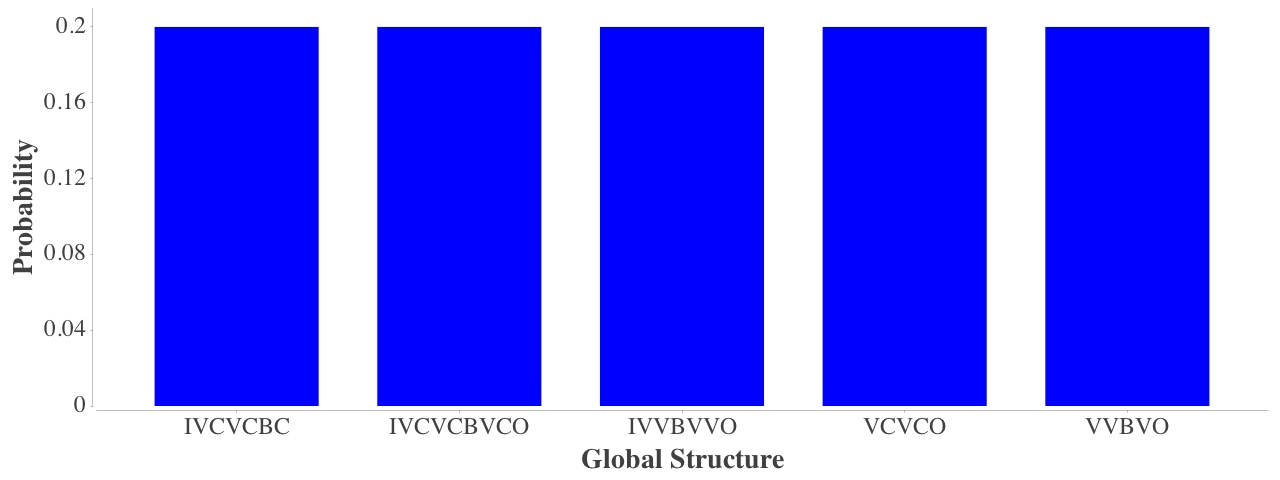
\includegraphics[width=\linewidth]{global_structure}
	\caption{\label{fig:global_structure} A visual representation of a possible probability distribution over global song structures composed of verses (V), choruses (C), intros (I), outros (O), and bridges (B).}
\end{figure}

A second approximation is a \textit{distributional model} which learns a multinomial distribution of possible structures from a corpus of composition artefacts (e.g., see Figure~\ref{fig:global_structure}). The disadvantage to the distributional model is that it can only produce structures seen in training. 

A third, more powerful approximation uses a \textit{constrained Markov model}. This model factors $P(\zeta|\nu)$ into a distribution over the number of segments in a song, $P(|\zeta|)$, and a single-order Markov model for sequences of segment types:
\[ P(\zeta|\nu) = P(|\zeta|) P(\zeta_1) \prod_{i=2}^{|\zeta|} P(\zeta_i|\zeta_{i-1}) \]
\noindent Note that an unconstrained, unsmoothed Markov model for $P(\zeta_i|\zeta_{i-1})$ provides no guarantee that a sequence of length $|\zeta|$ can or will be generated, nor that the sequence will end naturally (e.g., with an outro). With \citeauthor{pachet2001finite}'s \emph{constrained} Markov model we can constrain the length and the way the sequence ends. This modifies the way $P(\zeta|\nu)$ is factored by conditioning $\zeta_i$ on both $i$ and $\zeta_{i-1}$:
\[ P(\zeta|\nu) = P(|\zeta|) P(\zeta_1) \prod_{i=2}^{|\zeta|} P(\zeta_i|i,\zeta_{i-1}) \]
When generating, a length is sampled from $P(|\zeta|)$ and a constrained Markov model for the sampled length is constructed from the unconstrained model $P(\zeta_i|\zeta_{i-1})$ with the added constraint that the song must end on an ``end'' token. This model is capable of creating sensible structures of reasonable length that were not seen in the training data. Empirical distributions for approximating $P(|\zeta|)$ and $P(\zeta_i|\zeta_{i-1})$ are shown in Figures~\ref{fig:segment_count_per_song} and~\ref{fig:segment_transitions} respectively.

A fourth possible solution for generating global structure would be to use a generative grammar, learned or manually constructed, similar to what was done by \cite{steedman1984generative}.

\begin{figure}
	\centering
	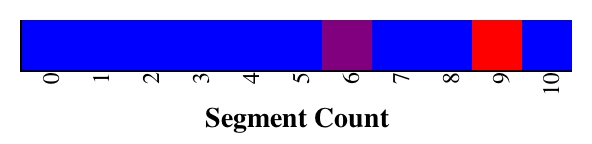
\includegraphics[width=.8\linewidth]{segment_count_per_song}
	\caption{\label{fig:segment_count_per_song} A visual representation of a possible probability distribution over the number of segments per song. Red corresponds to high probability, blue to low.}
\end{figure}

\begin{figure}[t]
	\centering
	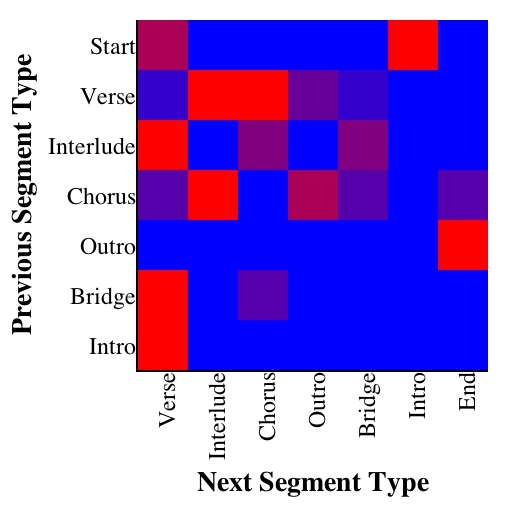
\includegraphics[width=.6\linewidth]{segment_transitions}
	\caption{\label{fig:segment_transitions} A visual representation of a possible single-order Markov transition matrix for segment types. Red corresponds to high probability, blue to low. The results largely agree with intuition. For example, songs generally start with an intro and occasionally with a verse; songs generally end with an outro and occasionally a chorus; and segments of the same type do not generally follow one another.}
\end{figure}

In addition to global structure, we also model \emph{segment structure}, $P(\sigma|\nu,\zeta)$. Though this segment structure could be included as part of global structure, modeling this substructure independently leverages principles of abstraction and polymorphism in order to facilitate novel combinations of substructures. For example in story-generation the global structure might dictate something about the abstract content of each paragraph (e.g., protagonist faces a trial, protagonist learns lesson, etc.), whereas the segment structure might define the narrative style for the paragraph (e.g., dramatic visualization, retrospection, dialogue, etc.) or add definition to the abstract content (e.g., the trial is a storm, the trial is losing a loved one, etc.). Modeling these structures independently enables the model to combine narrative styles with plot elements in ways that were not seen during training.

A segment in a composition (e.g., a verse) exhibits structure in the number of measures, the number of syllables or notes per segment, which lyrics rhyme or repeat, and patterns in harmony, pitch, or rhythm. We define a segment structure for lyrical composition as a sequence of pairs $\sigma = ((l_1,C_1),\mydots,(l_{|\zeta|},C_{|\zeta|}))$, where $l_i$ is the measure length of the $i$th segment (corresponding to $\zeta_i$) and $C_i = \{{c_{i1},\mydots,c_{in}}\}$ is a set of constraints which apply to the $i$th segment.

Constraints define restrictions on different musical viewpoints in order to create rhyme and repetitive motifs. A constraint, $c_{ij}$, is defined for a particular viewpoint $v\in\{Harmony, Pitch, Rhythm, Lyric\}$; with a condition $d\in\{Equals, Matches, RhymesWith, HasExpectation\}$; with a Boolean value $t$ that defines whether the condition $d$ needs to be satisfied or unsatisfied in order to satisfy the constraint $c_{ij}$; and with $m\in[0,l_i)$ and $b\in[0.0,bpm_m)$ representing the measure and beat offset within the segment to which the constraint applies ($bpm_m$ is the beats per measure of $m$). Each condition $d$ has different sub-variables and dimensionality:

\begin{itemize}
\item $Equals$ conditions - $c_{ij} = (v,d=Equals,t,m,b,S)$, where to satisfy $d$, the $v$ token at or near measure $m$, beat $b$ must equal a $v$ token in the set of tokens $S$ if $t$ is $true$ and must not equal any $v$ token in $S$ if $t$ is $false$.
\item $Matches$ conditions - $c_{ij} = (v,d=Matches,t,m,b,$ $m_2,b_2)$, where to satisfy $d$ the $v$ token at or near measure $m$, beat $b$ and at or near measure $m_2$, beat $b_2$ within the segment must be equal if $t$ is $true$ and not equal if $t$ is $false$.
\item $RhymesWith$ conditions - $c_{ij} = (v=Lyric,d=Rhy\-mes\-With,t,m,b,m_2,b_2)$, where to satisfy $d$ the $Lyric$ tokens at or near measure $m$, beat $b$ and at or near measure $m_2$, beat $b_2$ within the segment must rhyme if $t$ is $true$ and not rhyme if $t$ is $false$.
\item $HasExpectation$ conditions - $c_{ij} = (v,d=HasEx\-pectation,t,m,b,s)$, where to satisfy $d$ the $v$ token at or near measure $m$, beat $b$ must have an expectation value above a threshold $s$ if $t$ is $true$ and not have an expectation value above $s$ if $t$ is $false$. This constraint can be used to create a structure of expectation (as discussed by \citeauthor{meyer2008emotion} \shortcite{meyer2008emotion}) in order to model patterns of surprise and tension.
\end{itemize}

Note that the attribute $t$ could allow the system to learn how to intelligently break rules. For example, the system could intelligently learn when \emph{not} to rhyme when perhaps a rhyme would normally be expected.

We define the distribution over segment structures $\sigma$ as
\[ P(\sigma|\nu,\zeta) =  \prod_{i=1}^{|\zeta|} P(C_i | l_i) P(l_i|\zeta_i). \]

To approximate $P(l_i|\zeta_i)$ we can learn a probability distribution over segment lengths conditioned on segment type (see Figure~\ref{fig:measure_count_by_segment}). Under the assumption that the constraint set for a segment is independent of the segment type given its length, we can approximate $P(C_i | l_i)$ using a probability distribution over sets of constraints conditioned on segment length (e.g., see Figure~\ref{fig:segment_structure}).

\begin{figure}[t]
	\centering
	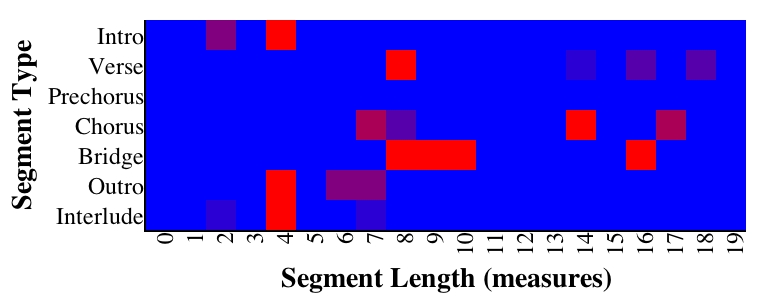
\includegraphics[width=\linewidth]{measure_count_by_segment}
	\caption{\label{fig:measure_count_by_segment} A visual representation of an empirically derived probability distribution over song segment lengths, conditioned on segment type. Red corresponds to high probability, blue to low. The results largely agree with intuition: intros, outros, and interludes tend to be shorter; verses, bridges and choruses tend to be longer.}
\end{figure}

\begin{figure}[t]
	\centering
	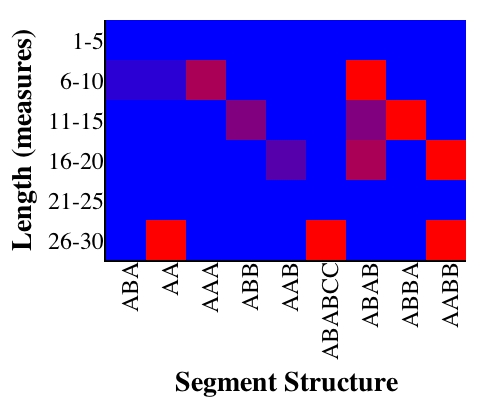
\includegraphics[width=.7\linewidth]{segment_structure}
	\caption{\label{fig:segment_structure} A visual representation of an empirically derived probability distribution over song segment rhyme structures conditioned on segment length. Red corresponds to high probability, blue to low.}
\end{figure}

Much of the work that has been done with finite-length Markov processes with constraints has required the user to specify the desired constraints in the composition process (e.g., \cite{pachet2014imitative,barbieri2012markov}). This step of learning a model of constraints gives the system increased autonomy to choose its \emph{own} constraints and then generate artefacts to meet those constraints.

With regard to modeling distributions for implicit features of an artifact (e.g., rhyme constraints), empirically-derived distributions can incur significant AI challenges. Artefacts used for training often fail to label global and even segment structure, and therefore these implicit features must be manually labeled or somehow inferred. Though our current system learns structure from a small manually-annotated dataset, our goal in future work is to use sequence alignment over multiple viewpoints to infer global structure, finding regions of a composition where harmony, melody, and lyrics all match (i.e., chorus) or where only harmony and melody match (i.e., verse). Sequence alignment is also a promising approach to finding segment structure (e.g., \citeauthor{hirjee2010using} \shortcite{hirjee2010using} use alignment to detect rhyme scheme).

Having modeled the abstract structural representation, the system proceeds to model the \emph{operational} representation of the artefact (e.g., paint strokes, narrative text, recipe ingredients, etc.). Whether modeled jointly or factored, the operational variables describing the artefact composition are conditioned on the constraints imposed by the intention and global/segment structure. Adapting Pachet and Roy's definition of a jazz leadsheet (\citeyear{pachet2014imitative}), we define the operational representation of a lyrical composition as parallel sequences of chords $\eta$, notes $\mu$, and lyrics $\lambda$ each with the same total duration. $\eta$, $\mu$, and $\lambda$ are defined in the following sections.

\subsubsection{Harmony, $P(\eta|\nu,\tau)$}

We define a harmony as a sequence of positioned chords $\eta = (C_1,\mydots,C_n)$ of arbitrary length. Each positioned chord $C_i = (I_i,d_i)$ has an identity $I_i = (r_i,q_i,s_i)$, with root pitch $r_i\in[0,11]$, chord quality $q_i$ (e.g., major, minor, dominant, etc.\footnote{possible values for $q_i$ are defined according to the MusicXML 2.0 specification for chord qualities}), and bass pitch $s_i\in[0,11]$; and a duration $d \in \mathbb{R}_{>0}$. We normalize all root and bass pitches based on the labeled key signature of the training instance at the harmony position.

\begin{figure}[t]
	\centering
	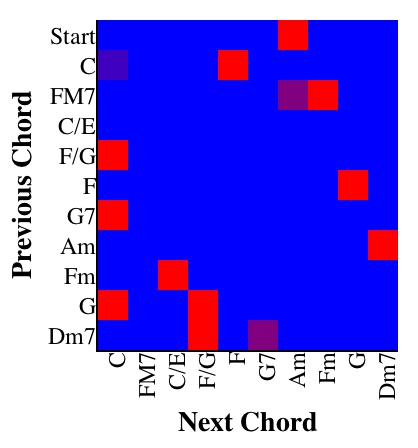
\includegraphics[width=.6\linewidth]{harmony}
	\caption{\label{fig:harmony} A subsection of a visual representation of an empirically derived single-order Markov transition matrix for harmonic chord sequences for chorus segments. Red corresponds to high probability, blue to low. As expected for songs normalized to the key of C major, there is high probability that the song starts on a C major chord. }
\end{figure}

We can factor $P(\eta|\nu,\tau)$ into independent sequential models regulating chord duration and chord identity:
\small
\[ P(\eta|\nu,\tau) = P(I_1|\tau) P(d_1|\tau) \prod_{i=2}^n P(I_i|I_{i-1},\tau) P(d_i | d_1,\mydots,d_{i-1},\tau). \]
\normalsize
\noindent  In this formulation, the length of the sequence $n$ is dynamically determined such that $\Sigma_{i=0}^n d_i$ equals the segment duration.

Deciding how to implement $P(I_i|I_{i-1},\tau)$ and $P(d_i | d_1,\mydots,d_{i-1},\tau)$ is non-trivial. A few possibilities for probabilistic sequence models include:
\begin{enumerate}
\item a \textit{fixed generator} generates a fixed token, essentially ignoring conditioned variables
\item \label{model:distribution_model}a \textit{probability distribution} over tokens, conditioned on segment type and/or beat position, but not previous token
\item a \textit{Markov model} that generates a new sequence for each segment, independent of segment type
\item \label{model:seg_model}a \textit{set of Markov models} - one model per segment type
\item a \textit{hidden Markov model} - hidden states representing the segment type
\end{enumerate}
\noindent Each model has limitations that must be considered in the context for which it is intended. Of these, our implementation uses model~\ref{model:seg_model} for $P(I_i|I_{i-1},\tau)$ (see Figure~\ref{fig:harmony}) and model~\ref{model:distribution_model} for $P(d_i | d_1,\mydots,d_{i-1},\tau)$ (for a discussion of the relative musical merits of these models see \citeauthor{bodily2017Mume} \shortcite{bodily2017Mume}).

The decision to assume that duration and chord are independent, though potentially erroneous, is deliberate. This is based on the reasoning that the strength of a probabilistic model depends on the number of instances used to train the model. Each time a distribution adds a conditional variable, the power of the model is reduced. We feel that the duration and chord are sufficiently independent that the model strength recovered by assuming independence outweighs the cost of ignoring any dependence between them.

\subsubsection{Melody, $P(\mu|\nu,\tau,\eta)$}

A melody is a sequence of positioned notes $\mu=(N_1,\mydots,N_n)$ of arbitrary length. Each note $N_i = (p_i,d_i)$ has a pitch $p_i\in[-1,127]$  (corresponding to a MIDI note value, -1 representing a rest) and a duration $d_i \in \mathbb{R}_{>0}$. We factor $P(\mu|\nu,\tau,\eta)$ into independent sequential models regulating note pitch and duration:
\small
\[ P(\mu|\nu,\tau,\eta) = P(p_1|\eta) P(d_1|\tau) \prod_{i=2}^n P(p_i|p_{i-1},\eta) P(d_i|d_{i-1},\tau). \]
\normalsize
\noindent The length of the sequence $n$ is dynamically determined such that $\Sigma_{i=0}^n d_i$ does not exceed the segment duration.

Of these models only pitch is conditioned on $\eta$. To model $P(p_i|p_{i-1},\eta)$ our implementation uses a single-order Markov chain of scale steps where the scale is defined by the contextual harmony of $\eta$. To model $P(d_i|d_{i-1},\tau)$ we use a segment-specific Markov chain of note durations (see Figure~\ref{fig:melody_rhythm}). Any of the probabilistic sequence models considered for harmony could also be considered here.

\begin{figure}[t]
	\centering
	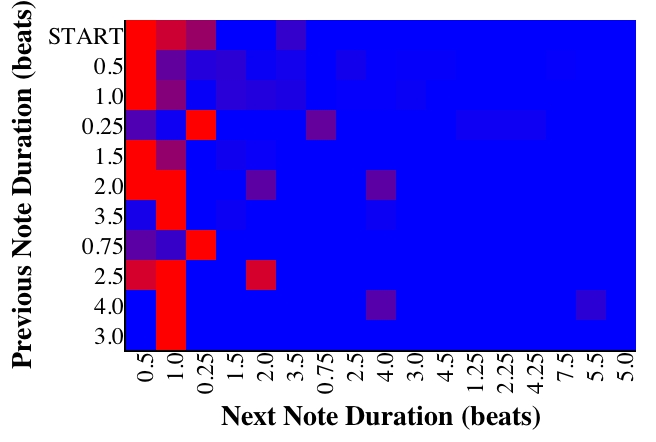
\includegraphics[width=\linewidth]{melody_rhythm}
	\caption{\label{fig:melody_rhythm} A visual representation of an empirically derived single-order Markov model for melodic rhythm durations for verse segments in 4/4. Red corresponds to high probability, blue to low.}
\end{figure}

\subsubsection{Lyrics, $P(\lambda|\nu,\tau,\mu)$}

Several models of natural language generation (NLG) and in particular NLG in poetry and music have been published \cite{paris2013natural}. As these models continue to improve, so will their application in lyrical composition. This demonstrates the robustness of the HBPL framework: as improved submodels are conceived and implemented, the joint model is also improved.

We define lyrics as a sequence of stressed syllables $\lambda=(S_1,\mydots,S_n)$ where $|\lambda| \le |\mu|$. A stressed syllable $S_i = (t_i, p_i, \epsilon_i)$ has a text representation $t_i$, a pronunciation $p_i$ (e.g., sequence of ARPAbet phonemes), and a stress $\epsilon_i\in[0,2]$. Each syllable $S_i\in\lambda$ corresponds to one and only one note $N_j\in\mu$.
\begin{figure*}
	\centering
	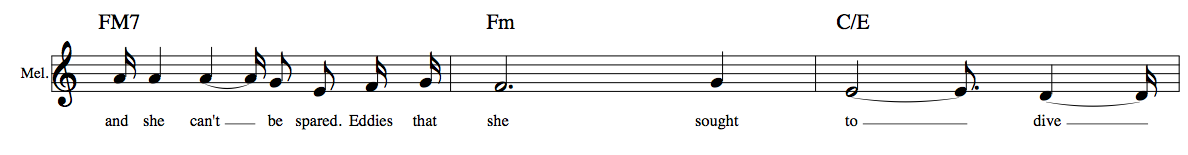
\includegraphics[width=\linewidth]{example}
	\caption{\label{fig:example_composition} Three measures of a sample composition generated using the HBPL framework. The full composition and others can be found online at \url{popstar.cs.byu.edu}.}
\end{figure*}

We factor $P(\lambda|\nu,\tau,\mu)$ to construct $\lambda$ as a sequence of lyric phrases $(\phi_1,\mydots,\phi_n)$ where the number of phrases $n$ and the length $l_{\phi_i}$ (in syllables) of each phrase are computed as a function of the notes in $\mu$ and the rhyme constraints in $\tau$ (i.e., we assume rhyme constraints denote phrase endings):
\[ P(\lambda|\nu,\tau,\mu) = \prod_{i=1}^n P(\phi_i | l_{\phi_i},\nu,\tau) P(l_{\phi_i} | \mu,\tau). \]
We empirically derive $P(l_{\phi_i} | \mu,\tau)$. For $P(\phi_i | l_{\phi_i},\nu,\tau)$ we create a probability distribution of lyric templates conditioned on $l_{\phi_i}$ which we use to sample templates. These templates, the $RhymesWith$ constraints of $\tau$, and $\nu$ are given as input to an independent module that generates novel, intentioned lyrics (see \citeauthor{bay2017ICCC} \shortcite{bay2017ICCC}). The module uses existing lyric segments as syntactic templates for the creation of novel lyric segments. It intelligently selects and replaces words based on 1) semantic similarity, 2) part-of-speech tag, 3) the cultural and thematic intention of $\nu$, and 4) the rhyme constraints imposed by $\tau$.

The advantage of using a template-based approach to lyrics generation is that it maintains syntactic coherence. The primary shortcomings are that resulting lyrics provide limited syntactic novelty from the training data and make no inherent effort at providing global semantic cohesion.

\subsubsection{A Note on Constrained Markov Models}

\citeauthor{pachet2001finite}'s constrained Markov model requires that the length of the sequence be defined \emph{a priori} \shortcite{pachet2001finite}. One short-coming in our current implementation is that because we have included duration as part of the definition for both harmony and melody (rather than having each chord or note representative of a fixed duration as demonstrated by \citeauthor{pachet2014imitative} \shortcite{pachet2014imitative}) the length of a harmony or melody sequence depends on the durations of each sampled chord or note. While this violates the Markov property and prevents us from being able to effectively use constrained Markov models, we favor the current implementation for reasons related to data sparsity issues and the complexity of implementing higher-order constrained (hidden) Markov model. We hope in the future to overcome both of these hurdles and to shift to ``Markov-friendly'' definitions for melody and harmony in order to more fully incorporate the constraints defined in $\tau$ using constrained Markov or constrained hidden Markov models.

\section{Results and Discussion}

We present results of implementing the HBPL framework in the context of a discussion of some of the model's implications. We trained submodels on a small manually-annotated subset of the Wikifonia leadsheet dataset.

\subsection{Using the Joint as a Submodel}

Because of the hierarchical nature of HBPL, a joint model of an artefact class (e.g., the model of $P(\gamma|\iota)$ just described) can serve as a submodel for other models. For example, we define the joint probability distribution on inspirations $\iota$, compositions $\gamma$, and renderings $\rho^{m}$ as follows,
\[ P(\iota,\gamma,\rho^1, ..., \rho^m) = P(\iota)P(\gamma|\iota) \prod_{m=1}^M P(\rho^m|\iota,\gamma). \]
In essence we decompose a model of music \emph{creation} to individually model the inspiration for the artefact, the symbolic (abstract) representation of the artefact, and the concrete rendering of the artefact. 

\subsubsection{Inspiration, $P(\iota)$}

\emph{Inspiration} (i.e., the method for deriving intention) may be more closely related to an artist's or system's ``creative spark''. For example, observers often perceive greater creativity in artefacts which in some way relate to them or to their culture \cite{colton2008creativity}. In the joint probability distribution on inspirations $\iota$, compositions $\gamma$, and renderings $\rho^{m}$, we define $P(\iota)$ not as the distribution over intentions, but as the distribution over inspiring sources for the intention. In other words, not ``what was the artefact intended to communicate?'', but ``what was the inspiring \emph{source} for what the artefact intended to communicate?''

In general this demonstrates an unanticipated benefit of factorization: we can condition on any variable that could be argued to influence the artefact's creation. Many creative systems implicitly define inspiration based on the corpora that the data trains on. With the concept learning framework, we can model this attribute explicitly.

This represents an aspect not present in the model originally presented by Lake et al. \shortcite{lake2015human}: not only are we modeling \textit{what} artefacts can be generated, but also \textit{why} they are generated. One possible way to model inspiration is to use an observer's environment or culture as an inspiring source. Research in electroencephalogram-based affective computing (i.e., reading brain waves) suggests that computers may soon be able to perceive an observer's emotional state beyond those of their human counterparts \cite{volioti2016mapping}. Alternatively, inspiration could be modeled using sentiment analysis in a variety of online domains. We plan to explore models of inspiration further in future research.

\subsubsection{Rendering, $P(\rho^{m}|\iota,\gamma)$}

The example model $P(\gamma|\iota)$ described above defines symbolic lyrical compositions (i.e., a leadsheet). However, evaluating an abstract artefact generally requires a concrete rendering of the artefact, whose distribution we model as $P(\rho^{m}|\iota,\gamma)$. As a proof of concept, we implemented and trained the described HBPL model on a small corpus of hand-annotated lyrical pop composition data. To concretely render compositions created using this model, we generated both printed sheet music (e.g., Figure~\ref{fig:example_composition}) and an MP3 audio recording\footnote{audio recordings can be found at \url{popstar.cs.byu.edu}}. Our MP3 audio file features computer-sung lyrics accompanied by synthesized piano and bass comping chords\footnote{generated using Harmony Assistant (v9.7.0f) and Virtual Singer (v3.2)}.

\subsubsection{Implications for Recommendation Systems}

Lake et al. present the model of $P(\psi)$ given in equation \ref{eq:1} as a submodel of the factoring of the joint probability distribution on character types $\psi$, tokens $\omega^m$, and binary images $I^m$ \shortcite{lake2015human}:
\small
\[ P(\psi, \theta^1, \mydots,\theta^M,I^1,\mydots,I^M) = P(\psi) \prod_{m=1}^{M} P(I^m|\theta^m)P(\theta^m|\psi). \]
\normalsize
This means that given an image, the system can discover the motor program (i.e., abstract character type) that most likely generated it. This allows the system to one-shot classify and generate pairs of images that represent the same character type (specific examples of which were not seen in training). 

By analogy, a model for $P(\gamma)$ (similar to $P(\gamma|\iota)$ just described) could be inserted into a joint probability on composition types $\gamma$, arrangements $\alpha^m$, and audio recordings $\rho^m$,
\small
\[ P(\gamma,\alpha^1,\mydots,\alpha^M,\rho^1,\mydots, \rho^M) = P(\gamma) \prod_{m=1}^M P(\rho^m|\alpha^m)P(\alpha^m|\gamma). \]
\normalsize
The implications of this model are more broadly significant: the HBPL framework is capable of inferring abstract representations of concrete artefacts, representations which more directly define meaning, composition, and causality. This is significant for two reasons. First, in some realms of creativity, simply deriving the abstract representation of an artefact is valuable (e.g., automatically transcribing sheet music from audio). Second, having an abstract representation allows concrete artefacts to be compared according to symbolic, conceptual criteria (e.g., recommendation systems based on meaning, or in the case of music, harmony, melodic pitch or rhythm, etc.). Though work has been done to approximate $P(\alpha^m|\gamma)$ \cite{benetos2013automatic}, effective comparison of artefacts hinges on the other terms in the factorization, $P(\gamma)$ and $P(\rho^m|\alpha^m)$, which are lacking.

\subsection{Fitness and Self-Evaluation}

The HBPL framework is designed to restrict the generation process \emph{in situ} to produce only meaningful artefacts (as compared to a generate-and-test procedure). As discussed by \citeauthor{ventura2016mere} \shortcite{ventura2016mere}, this ``baked-in'' self-evaluation mechanism has the added benefit of being able to explain to some extent both the novelty, value, and motivation behind generated artefacts. Given its ability to compute probabilities, the HBPL framework could thus also be potentially leveraged as a fitness function for other types of generative models.

\subsection{Big (Need for) Data}

Any empirically-driven model requires training on a dataset representative of the artefact domain. Even if we had digital access to all of the compositions ever written, it would represent an infinitesimal portion of the songs that \emph{could} be written. This is a challenge in many machine learning domains. Unique to the pop music domain, however, is that data is highly proprietary. What \textit{is} available is extremely limited and of relatively poor quality. Compared to natural language, artefacts in music generally require relatively complex representations and relatively few possess the domain knowledge required to generate or transcribe the needed data. Among those who \textit{do} understand and use it, music formatting can vary wildly and inexactly---creating additional challenges for a by-the-bit computer parser. Computers will only learn to speak music as quickly as we either formalize and ubiquitize the language of music \textit{or} endow computers with AI tools to fill in the gaps on their own.

The particular challenge of accessing high-quality symbolic \emph{pop} music datasets is significant. There is a dearth of well-annotated resources for those interested in studying any or all of the aspects of pop music composition. There is, however, much we can do to improve the situation. First, we need to make resources that \textit{are} available more accessible (guitar tabs, lyrics sites, beatles). Second, we need to establish a better case for how society and industries stand to benefit from computational pop music research in order to generate a productive dialogue for the support and collaboration of those in possession of large pop music datasets (sheet music sites, spotify, etc., asking for APIs, etc). Note that this is different than asking them to simply give us their proprietary data. Third, we can do more to recognize contributions of novel datasets.

\section{Conclusion}

HBPL is a powerful framework for accomplishing tasks in computational creativity. Using principles of compositionality, causality, and learning-to-learn, such models are able to effectively learn and generate examples of complex creative concepts. Its probabilistic framework lends itself well to modeling important aspects of creativity such as inspiration and intention. The HBPL framework by nature compels researchers in domain-specific subareas of computational creativity to engage in the debates that the artists themselves are having, namely ``how should an artefact be created?'' and ``does it matter?'' To the extent that these challenges are effectively addressed on the scale of defining and training subconcept models, the HBPL model represents a useful framework for designing and assessing creative systems.

\bibliographystyle{iccc}
\bibliography{../all}

\end{document}
